\section{Security}
\label{security}

The goal of the proposed \ivfsystem{} is to facilitate reuse of the \projectdata{}.
There is, however, one major restriction with data sharing and re-use: medical data is (almost always) highly sensitive and must be secured. 
This imposes strong conditions for reusing the data, which have to be taken into account by the system.

Below we present the security study together with the drawn conclusions.
Literature was searched for security issues and solutions in systems used within the clinical domain.
The identified security aspects were applied to real-life examples gathered in an interview with a software engineer working on systems that support a large clinical data registry in The Netherlands.
The full security review and interview transcript can be found in appendix \ref{security-review-appendix}.

\paragraph{Security Analysis: the \ivfsystem{} case}
\label{security-summarisation-analysis}

\silvia{i think this is too vague. what are the issues and solutions?}
A multitude of security issues and solutions have been identified from the literature study.
As a general rule, exploring and using present day standard security measures are a must-have for a good system.
During the software engineering cycle of the \ivfsystem{}, the appropriate security measures for each part of the system will be identified and adopted.
Also the expertise of developers, engineers, and system administrators with multiple years of experience will be used for a proper system design.
In addition to this, there are a few highly important concepts of security, which are a mixture of technical, lawful, and ethical components.
These concepts are interesting to look at as they have a high impact on how data may be used.

The first aspect is "consent for data access", for the \project{} it can be viewed from multiple perspectives: patient, clinic, and registry.
When researchers want to use the dataset available in the \ivfsystem{}, they will use data coming from the clinics, which in turn gather data from patients.
This patient data is then linked to the PRN registry data.
Each of the parties involved should to some extent be able to determine if they allow their data to be used.

Patient consent is a difficult problem to tackle in research in general.
When giving consent, patients need to know what they are signing for. Moreover, handling data outside of the goal which was described is forbidden.
However, there are exceptions in the Dutch consent regulations 
when using datasets for which it is unreachable and unreasonable to acquire consent from each patient in them.
This exception is what the \ivfsystem{} currently leans on. 
It uses historical data for the years 2000 to 2010 and, according to the nationwide IVF report \cite{ivfReportNVOG}, there are approximately 4000 pregnancies per year.
This means that there are about 40.000 patients in the dataset in total, so 
given the size and age of the dataset it was deemed unreasonable to require consent.
To determine if consent is not a requirement, advice from external parties should be acquired.
In this case these were the \AMC{} chief privacy officer, the medical ethical committee of data suppliers, and the \PRN{} privacy committee.

Consent from clinics and registries can be compared to patient consent.
They all give permission to use \emph{their} data for a specific cause as described in the consent.
The main difference between these data providers in giving consent is that their considerations are based on different interests.
For example, a patient might be concerned about his/her privacy.
Of course a clinic will also take this into account when a dataset is requested, but they also have interests in the type of research to be performed with the data.
If this clashes with a research interest of their own, it is less likely the clinic will give consent.
In the \ivfsystem{} these different levels of consent must be taken into account  to be able to perform the function of providing research data to answer new research questions.

In order to fulfil regulations and ethical needs a dataset should be minimised, so that no superfluous items are left in the dataset.
A purpose should be described for each of the data items in the dataset. 
This purpose description is essential to support ethical discussions about whether to deliver a data item in the dataset or not.
Having a well-defined protocol with the \ivfsystem{} can provide more confidence in the system by users, leads to better understanding of the system, and provides evidence of which choices about data items were made within certain considerations.

For data linkage some identifying (\ie{} private) data items are needed.
This can be described in the purpose of the data item, but there are also methods for avoiding these data items.
Hashing of data with the application of Bloom filters \cite{s22schnell2009} makes it possible to link two datasets without revealing the identifying data.
Online data linkage is only mentioned as a future work for the \ivfsystem{}.
In the first implementation, linkage is provided by a third-party and the delivery of linked data itself is seen as an offline external component of the system.

Anonymisation and pseudonymisation should be used to de-identify individuals.
While identification through data aggregation and cross-referencing is still possible to happen, these steps should make it more difficult.
The \ivfsystem{} will use both techniques to provide privacy. Datasets are mostly kept clean by removing all identifying data at the data gathering step.
And whatever identifying data is left (through linkage) will be pseudonymised before it is accepted into the system.

In order to decrease the chances of cross-referencing and data breaches in general, auditing should be applied.
This means keeping logs on who uses what data at what point in time and what version of data existed at that time.
Apart from privacy, this also makes it possible to keep people accountable and to provide research data management functionalities such as archival and provenance.

\paragraph{Provenance and the \ivfsystem{}}
If the reasoning is flipped over it can also be said that provenance provides data auditing capabilities.
A short review on the subject is provided in appendix \ref{provenance-review-appendix}.
The essence of provenance is to store metadata about the `life' of a piece of data (where does it come from, how was it processed, etc.).
This metadata can be used to create a view for human consumption as described by the PROV Model Primer \cite{dsp8gil} published by the W3C (World Wide Web Consortium\footnote{http://www.w3.org/}).
An example of human consumable provenance is shown in figure \ref{fig:provenance-schema-text}.

There are many applications of provenance in security, and  different levels can be supplied by mixing computerised surveillance with human insight.
One of the clearest examples is  data auditing.
The necessary metadata for an audit is collected automatically during the operation of the system.
Outcomes of this audit can be partly analysed by a computer, but can also additionally be translated into an human readable format.
Further actions that lead to actual security \silvia{??} should be captured in standardised processes, therefore provenance is only a tool and not a security end-point.

\begin{figure}[h]
	\centering
	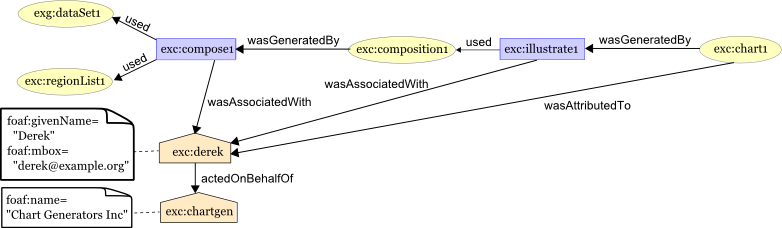
\includegraphics[width=1.0\linewidth]{images/provenance-large-schema}
	\caption{
		This example describes the creation of a chart, the original data used, the intermediate data generated during the process, the used software, who was responsible for the work, and who this person was working for.
		Taken from PROV Model Primer \cite{dsp8gil}.
		Detailed description can be found in appendix \ref{provenance-review-appendix}.
	}
	\label{fig:provenance-schema-text}
\end{figure}